% !TEX TS-program = LuaLaTeX

\documentclass{coderdojo}

\worksheet{11}{Cellular Automaton}

\newcommand\contentsitem[2]{
	\item \hyperref[#1]{\color{section}\bfseries #2}
}

\usepackage{wrapfig}
\usepackage{float}

\newcommand\TODO[1]{
\begin{itemize}
\item[\todoSymbol] \color{todo} #1
\end{itemize}}


\newcommand\TEST[1][\bf Test your code!]{
	\centerline{\tikz\node[starburst, fill=yellow, draw=red, line width=2pt,align=center] {#1};}
}

\newcommand\TESTSMALL[2][\bf Test your code!]{
{\tikz[scale=#2]\node[starburst, fill=yellow, draw=red, line width=2pt,align=center] {#1};}
}

\usetikzlibrary{decorations.pathreplacing}

\usepackage{cleveref}

\definecolor{state}{named}{blue}

\def\state#1{\textcolor{state}{\sf #1}}

%: DOCUMENT

\begin{document}

\maketitle

\section*{Introduction}

\begin{minipage}{.5\textwidth}
Imagine a fire in a forest, like that shown in the satellite image. If we know where the fire started, then
\begin{itemize}
\item in what direction is it likely to burn?
\item what is the probability of the fire consuming the entire forest?
\item how few trees do we need to fell to be sure that a single fire will not  consume the entire forest?
\end{itemize}
\end{minipage}
\begin{minipage}{.48\textwidth}\centering
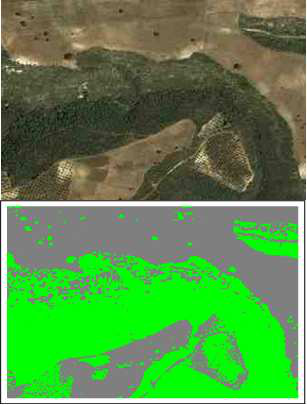
\includegraphics[width=.85\textwidth,clip,trim=0 205 0 0]{forest}
\end{minipage}

\vspace{3pt}
Or consider the spread of an infectious disease in a city --- will everybody get ill?
Or consider the spread of a rumour in the school yard --- how soon until everybody hears the rumour?

\vspace{6pt}
All three problems, seem very different, but all can be studied using {\em Cellular Automaton}.

\begin{exercise}[title=Cellular Automaton]

\begin{itemize}
\item 
We take our world (the forest) and split it into separate regions, called {\em cells}.
\item
Each cell is treated as a single unit, and is classified in a fixed set of {\em states}. For example, in a forest fire model each cell is classified as
\[
	{\mathrm {states}} = \{\state{unburnable}, \state{burnable}, \state{burning}, \state{burnt}\}
\]
\item 
We need a set of rules that describe how the state of the cells change in response of their current state and the state of their neighbouring cells.

For example, in a forest fire model:
\begin{itemize}
\item
a cell can change from state \state{burnable}\ to \state{burning}, when fire spreads from a neighbouring cell, but cannot change to states \state{unburnable} or \state{burnt}.
\item
a cell can change from state \state{burning}\ to \state{burnt}, when all the fuel (trees) in the cell are consumed, but cannot change to states \state{unburnable} or \state{burnable}.
\end{itemize}

\item
Finally we setup our model with some initial conditions (say, a fire in a random cell), and we get the computer to do the work of simulating what will happen over time. 
\end{itemize}
\end{exercise}


\vfill
Some of the material covered here came from the following paper, but google "cellular automation applications" for more example, in particular search for the Game of Life.

\begin{itemize}
\item  {\bf A Cellular Automata Model for Fire Spreading Prediction}\\
by {Quartieri, J. and Mastorakis, Nikos and Iannone, Gerardo and Guarnaccia, Claudio.}
{International Conference on Urban Planning and Transportation}, 2010.

\end{itemize}

\section{Before we start \ldots}

We need to install two python packages before we can start our simulation. The two packages are:
\begin{itemize}
\item \code{numpy}\\
This is a replacement for python lists, that can run up to 100s of times faster.  
This is important in cellular automation where we want lots of cells. 
\item \code{matplotlib}\\
This is a library for drawing graphs, we could use \code{turtle} package for this but \code{matplotlib} will make our life easier.
\end{itemize}

\TODO{Installing packages on Thonny}{

To install a python package in Thonny, select menu option \code{Tools}$\to$\code{Manage Packages..}. Then:
\begin{enumerate}
\item Enter the package name in the search box (\code{numpy} or \code{matplotlib}).
\item Click on \code{Search}.
\item An \code{Install} button should appear and click on this.
\item When installed both packages, exit by clicking on \code{close}.
\end{enumerate} 

\centerline{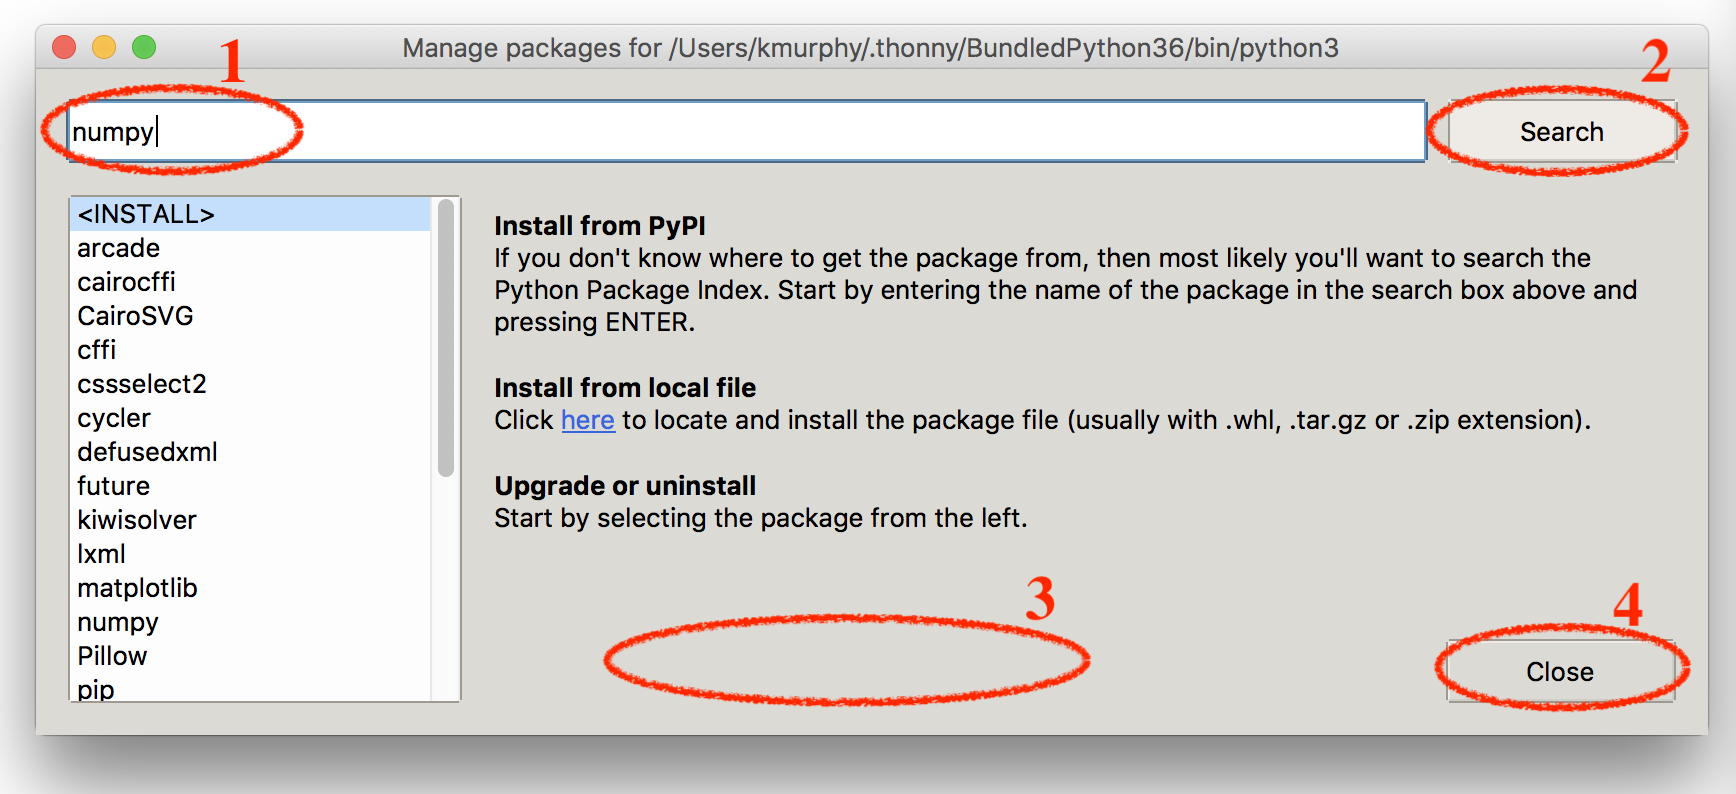
\includegraphics[width=0.8\textwidth,clip,trim=33 56 22 0]{thonny_packages.png}}}

\TODO{To check that the installation of the packages worked, type in the following program and verify the output.}
{All this code does in create a world consisting on $1\times 1$ cells, and displays it.  
%We will talk about what the code is doing soon, but for now we just want to verify that things work.
}

\codeandoutput{title={\code{test_packages.py}}}{1}{20}{code/public}{test_packages.py}{

	\centering	
	\tikz\node[fill=white]{
	\includegraphics[clip,trim=0 10 0 10, width=\textwidth]{code/output/test_packages.pdf}};
}


\section{One-Dimensional (1D) Cellular Automation}

Before we get to the forest fire model we will use the following simpler problem to introduce the main concepts.

\def\bulbOFF{
\includegraphics[height=1cm,clip,trim=0 10 170 0]{blub}}
\def\bulbON{
\includegraphics[height=1cm,clip,trim=170 10 0 0]{blub}}

\begin{exercise}[title=Line of Bulbs]
Consider a line of bulbs. Each bulb can be either off or on --- i.e. in cellular automation terms, each bulb is in one of two {\bf states}. One possible configuration of states is shown below:

\centerline{
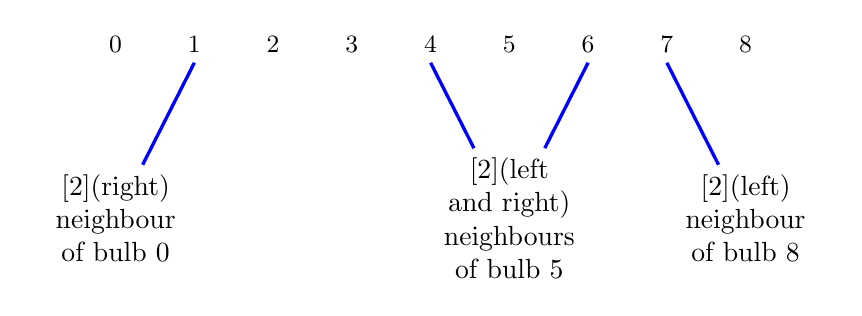
\begin{tikzpicture}
	\tikzstyle{note} = [font={\smaller[2]},text width=2cm, align=center]
	\tikzstyle{link} = [very thick, blue]
	%\node at (\x,0) (\x) {\bulbOFF}
	\foreach[count=\c] \x in {0,0,0,0,1,0,0,0,1} {
		 \node at (\c,0) (\c) {\ifnum\x=0\bulbOFF\else\bulbON\fi};  
		 \node at (\c,0.2) (\c) {\small \pgfmathparse {\c-1}\pgfmathprintnumber{\pgfmathresult}}; 
	}
	\node[note] at (1,-2) (N1) {(right)\\ neighbour of bulb 0};
	\node[note] at (9,-2) (N3) {(left)\\ neighbour of bulb 8};
	\node[note] at (6,-2) (N2) {(left and right)\\ neighbours of bulb 5};
	\draw[link] (N1) -- (2.270);
	\draw[link] (N2) -- (5.270);
	\draw[link] (N2) -- (7.270);
	\draw[link] (N3) -- (8.270);
%\bulbOFF\bulbOFF\bulbOFF\bulbOFF\bulbON\bulbOFF\bulbOFF\bulbOFF\bulbOFF
\end{tikzpicture}
}

Every day we update each bulb, turning it off or on, or leaving it unchanged based on its current state and the state of its neighbours --- this is our {\bf update rule}.

Depending on the update rule, over time which bulbs are on and which bulbs are off?

\end{exercise}

\subsection{Before we try to tell a computer to \ldots}

In programming circles you often hear the advice "before we try to tell a computer to do something we should make sure that we understand exactly what we are trying to do". So let us think about this problem by hand first.

\TODO{So consider both of the following and colour the bulbs that are on each day according to the given rules. (The first example is half-done to get you started.)}

\newcommand\model[2]{
	\pgfmathsetmacro{\d}{-1.6 * #1}
	\node at ($(0,\d)+(-.5,-0.)$) {\smaller Day {#1}};
	\foreach[count=\c] \x in {#2} {
		 \node at (\c,\d) (\c) {\ifnum\x=0\bulbOFF\else\bulbON\fi};  
		 \node at ($(\c,\d)+(0,0.2)$) (\c) {\smaller[2] \pgfmathparse {\c-1}\pgfmathprintnumber{\pgfmathresult}}; 
	}
}
\tikzstyle{example}=[fill=blue!5,drop shadow,rounded corners=6pt]
\tikzstyle{rule}=[fill=green!5,drop shadow,rounded corners=6pt,text width=7cm, font=\smaller,
	anchor=south west, xshift=-0.8cm,yshift=0.8cm]

\tikz\node[example]{
\begin{tikzpicture}[scale=0.7]
\node[rule] {Leave on any bulb that is on, and turn on any bulb that has at least one neighbour that is on.};
\model{0}{0,0,0,0,1,0,0,0,0}
\model{1}{0,0,0,1,1,1,0,0,0}
\model{2}{0,0,1,1,1,1,1,0,0}
\model{3}{0,0,0,0,0,0,0,0,0}
\model{4}{0,0,0,0,0,0,0,0,0}
\model{5}{0,0,0,0,0,0,0,0,0}
\model{6}{0,0,0,0,0,0,0,0,0}
\end{tikzpicture}};
%
\hfill
%
\tikz\node[example]{
\begin{tikzpicture}[scale=0.7]
\node[rule] {Turn on any bulb that has at least one neighbour that is on. If a bulb is on, then turn it off.};
\model{0}{0,0,0,0,1,0,0,0,0}
\model{1}{0,0,0,0,0,0,0,0,0}
\model{2}{0,0,0,0,0,0,0,0,0}
\model{3}{0,0,0,0,0,0,0,0,0}
\model{4}{0,0,0,0,0,0,0,0,0}
\model{5}{0,0,0,0,0,0,0,0,0}
\model{6}{0,0,0,0,0,0,0,0,0}
\end{tikzpicture}};

\clearpage
\TODO{Colour the bulbs that are on each day according to the given rules.}

\tikz\node[example]{
\begin{tikzpicture}[scale=0.7]
\node[rule] {Bulb is on if right neighbour is on, otherwise bulb is off.};
\model{0}{0,0,0,0,1,0,0,0,0}
\model{1}{0,0,0,0,0,0,0,0,0}
\model{2}{0,0,0,0,0,0,0,0,0}
\model{3}{0,0,0,0,0,0,0,0,0}
\model{4}{0,0,0,0,0,0,0,0,0}
\model{5}{0,0,0,0,0,0,0,0,0}
\end{tikzpicture}};
%
\hfill
%
\tikz\node[example]{
\begin{tikzpicture}[scale=0.7]
\node[rule] {Bulb is on if left neighbour is on, otherwise bulb is off.};
\model{0}{0,0,0,0,1,0,0,0,0}
\model{1}{0,0,0,0,0,0,0,0,0}
\model{2}{0,0,0,0,0,0,0,0,0}
\model{3}{0,0,0,0,0,0,0,0,0}
\model{4}{0,0,0,0,0,0,0,0,0}
\model{5}{0,0,0,0,0,0,0,0,0}
\end{tikzpicture}};

\vfill

Notice that, the bulbs at either end have only one neighbour. This becomes important for some rules. For example, in the following example we only update the bulbs in the middle because the rule does not make sense at either end. 

\vfill

\centerline{\tikz\node[example]{
\begin{tikzpicture}[scale=0.7]
\node[rule,text width=12cm] 
{Turn on any bulb that has exactly on one neighbour that is on, otherwise turn bulb off.};
\model{0}{0,0,0,0,0,0,0,0,1,0,0,0,0,0,0,0,0}
\model{1}{0,0,0,0,0,0,0,0,0,0,0,0,0,0,0,0,0}
\model{2}{0,0,0,0,0,0,0,0,0,0,0,0,0,0,0,0,0}
\model{3}{0,0,0,0,0,0,0,0,0,0,0,0,0,0,0,0,0}
\model{4}{0,0,0,0,0,0,0,0,0,0,0,0,0,0,0,0,0}
\model{5}{0,0,0,0,0,0,0,0,0,0,0,0,0,0,0,0,0}
\model{6}{0,0,0,0,0,0,0,0,0,0,0,0,0,0,0,0,0}
\model{7}{0,0,0,0,0,0,0,0,0,0,0,0,0,0,0,0,0}
\model{8}{0,0,0,0,0,0,0,0,0,0,0,0,0,0,0,0,0}
\model{9}{0,0,0,0,0,0,0,0,0,0,0,0,0,0,0,0,0}
\end{tikzpicture}};}




% line of 9 bulbs, with only the middle bulb on initially. Every day you enter the room with the bulbs and for each bulb you carry out the following rules:


\subsection{Step 0 --- Import the desired packages}

\TODO{Create a new file \code{bulbs_1d.py} and enter the following code.}

\codeonly{title={\code{bulbs_1d.py}}}{1}{3}{code}{bulbs_1d.py}  

The first two line load the two packages that we installed earlier, \code{numpy} and \code{matplotlib}, and we give then shorter names of \code{np} and \code{plt} to make life easier for us later.  
The third line loads a function used to set the colours to indicate a bulb is off (black) or on (yellow). 

\vspace{-6pt}

\subsection{Step 1 --- Create world}

\TODO{Let us assume we have 9 bulbs --- we can change this later --- then append the following code to \code{bulbs_1d.py}}

\vspace{-6pt}
\codeonly{title={\code{bulbs_1d.py}}}{5}{13}{code}{bulbs_1d.py}  

\begin{itemize}
\item
In line 6, we store the number of bulbs in variable \code{n}, this will make things easier later when we want to change the number of bulbs later.
\item
In lines 7, 8 and 9, we define the states that we need. Here \code{off=0} and \code{on=1}, and the colours used to represent them.
\item
In line 11, we allocate space to store the states of the \code{n} bulbs. The function \code{np.zeros} creates a list of zero to the size we want. 
%\item
%In line 13, we output our model --- we should see a line of zero indicating all bulbs are off.
\end{itemize}

\vspace{-6pt}
\begin{figure}[H]
\begin{tikzpicture}
	\node at (0,0) (W) {\includegraphics[scale=0.8,page=2]{grids}};
	\node at (7,-2.) (M) {\includegraphics[scale=0.8,page=3]{grids}};
	
	\draw[blue,-latex,very thick] (W.south) to[out=-90,in=180] node[left,text width=4cm,xshift=-13pt] 
	{treat each bulb as\\ a separate cell} (M.190);
\end{tikzpicture}
\caption{A 1D cellular automation consists of a row of cells. Each cell is identified by its column number (like houses on a street), but starting from the left with cell zero. \newline If we ignore the start and end cells, then every cell has two neighbours, one to the left (the west neighbour) and one to the right (the east neighbour). And we can get the address of the neighbours by adding/subtracting 1.}
\label{fig:1d}
\end{figure}

\TODO{Run the above code and verify that we see a line of zeros.}

\subsection{Step 2 --- Initialise model}

At the start the middle bulb is on. This is called our {\bf initial conditions}.

\TODO{Append the following code to \code{bulbs_1d.py}, and run the above code and verify that we see a line of zeros, with a single one (bulb on) in the centre.}

\codeonly{title={\code{bulbs_1d.py}}}{15}{19}{code/public}{bulbs_1d.py}  


\subsection{Step 3 --- Display model}

\TODO{Append the following code to \code{bulbs_1d.py}, and run the program, you should see the graphic shown below.}

\codeonly{title={\code{bulbs_1d.py}}}{20}{27}{code/public}{bulbs_1d.py}  

\begin{itemize}
\item In line 21--24 we define a function to draw our model.  
\begin{itemize}
\item
Line 22, displays the contents of \code{model} using function \code{plt.imshow}. The function \code{plt.imshow} is a general image viewer function and takes lots of parameters. We will cover this in more detail later.
\item
Line 23, adds a title to the image.
\item
Line 24, displays the graphics and pauses for 1 second.
\end{itemize}
\item 
Line 26, tests our function (always a good idea) and shows the starting state for one second.
\end{itemize}
\begin{figure}[H]\centering
\includegraphics[scale=0.5]{code/output/1D_0000.pdf}
\caption{Start point (initial state) for bulbs --- only centre bulb is on.}
\end{figure}


\TODO{Modify the code so that the leftmost bulb and the right most bulb is also on. You should get the following graphic:
\begin{figure}[H]\centering
\includegraphics[scale=0.5]{code/output/1D_start_ends.pdf}
\caption{Centre bulb and both end bulbs are on.}
\end{figure} 
}



\subsection{Step 4 --- Run simulation}

Finally, we come to the simulation bit --- this is where our work to date will pay off and the computer now does all of the heavy work for us. 

\TODO{Append the following code to \code{bulbs_1d.py}}

\codeonly{title={\code{bulbs_1d.py}}}{28}{37}{code/public}{bulbs_1d.py}  

\begin{itemize}
\item
Lines 27 to 29 apply the rule. In this case we turn on a bulb when its two neighbours are different (i.e., one neighbour is off and the other neighbour is on).

\[
	\text{neighbours of cell $c$ are at}
	\underbrace{\text{address $c-1$}}_{\text{left neighbour (west)}}
	\text{and}
	\underbrace{\text{address $c+1$}}_{\text{right neighbour (east)}}
\]
Notice two important things of this step:
\begin{itemize}
\item
before we started to update each of the cells (stored in \code{model}), we first had to make a copy of their current state, and saved this to \code{current}.
\item
Our rule applies to cells with two neighbours --- so we don't update the leftmost and rightmost cells. 
\end{itemize}
\item
Lines 37 display the model and pauses for 0.1 seconds, before continuning the simulation.
\end{itemize}

\subsection*{Some Quick Check Puzzles}

\TODO{Save file as \code{bulbs_1d_do_nothing.py} and modify the rule so that the all we see is a single light bulb in the centre.}

\TODO{Save file as \code{bulbs_1d_one_right_only.py} and modify the rule so that the all we see is a single light bulb on moving to the right.}

\TODO{Save file as \code{bulbs_1d_one_left_only.py} and modify the rule so that the all we see is a single light bulb on moving to the left.}

\TODO{Save file as \code{bulbs_1d_grow.py} and modify the rule so that we see the number of bulbs on growing outwards from the centre.}

\TODO{Save file as \code{bulbs_1d_flash.py} and modify the rule so that we see the flashing bulbs on and off every day.}

\section{Storing History in 1D Cellular Automation}

Ok, we now have a working simulation now but it could be improved.  One improvement is that we could save the history of the bulbs every day and at the end display this history.  Showing the history would make it easier to track what is happening and allow us to test more complicated rules.

\vspace{-6pt}
\TODO{Save your \code{bulbs_1d.py} as \code{bulbs_1d_history.py} and insert the changes below.}

\vspace{-6pt}

\begin{minipage}{\textwidth}
\begin{tikzpicture}
\node[inner sep=0pt, outer sep=0pt] (P) 
	{\begin{minipage}{\textwidth}
	\codeonly{title={\code{bulbs_1d_history.py}}}{1}{49}{code/public}{bulbs_1d_history.py}
	\end{minipage}};
\tikzstyle{nn}=[anchor=north east, draw, fill=yellow!20, drop shadow,align=left]
\tikzstyle{ll}=[line width=3pt, blue, -latex]
\node[nn] at ($(P.east)+(0,8.4)$) (N) {number of days to run simulation.\\ The more days we simulate the more\\
history we need to remember};
\draw[ll] (N.west) -- ++(-6,0);
\node[nn] at ($(P.east)+(0,4.3)$) (N) {allocate space to store history};
\draw[ll] (N.west) -- ++(-2,0);
\node[nn] at ($(P.east)+(0,2.3)$) (N) {store initial state into history};
\draw[ll] (N.west) -- ++(-6,0);
\node[nn] at ($(P.east)+(0,-6.4)$) (N) {store model into history};
\draw[ll] (N.west) -- ++(-6,0);
\node[nn] at ($(P.east)+(0,-9)$) (N) {display history};
\draw[ll] (N.west) -- ++(-2,0);
\end{tikzpicture}
\vspace{-54pt}
\end{minipage}


\TODO{When you run your \code{bulbs_1d_history.py} program, you should see the sequence of images showing the daily state (bottom left) and finally the complete history (bottom right).}

\begin{tikzpicture}

\foreach \d in {0,1,2,...,7} {
	\node at (0,-\d) {\includegraphics[scale=0.5]{code/output/1D_000\d.pdf}};
}
\node at (10,-3.5) {\includegraphics[scale=0.7]{code/output/1D_history.pdf}};

\end{tikzpicture}


\subsection*{Some Quick Check Puzzles}
\TODO{Modify your \code{bulbs_1d_history.py} program, changing either the initial condition and/or the update rule to generate each of the following effects.

\noindent
\begin{tabular}{@{}ccc}
{\bf A} & {\bf B} &  {\bf C} \\
{\includegraphics[scale=0.4]{code/output/1D_history_A.pdf}} &
{\includegraphics[scale=0.4]{code/output/1D_history_B.pdf}} &
{\includegraphics[scale=0.4]{code/output/1D_history_C.pdf}} \\
{\bf D} & {\bf E} &  {\bf F} \\
{\includegraphics[scale=0.4]{code/output/1D_history_D.pdf}} &
{\includegraphics[scale=0.4]{code/output/1D_history_E.pdf}} &
{\includegraphics[scale=0.4]{code/output/1D_history_F.pdf}} \\
{\bf G} & {\bf H} &  {\bf I} \\
{\includegraphics[scale=0.4]{code/output/1D_history_G.pdf}} &
{\includegraphics[scale=0.4]{code/output/1D_history_H.pdf}} &
{\includegraphics[scale=0.4]{code/output/1D_history_I.pdf}} \\

\end{tabular}
}


%\section{Two-Dimensional (2D) Cellular Automation}

\end{document}
























The title of this worksheet is a little ambitious --- we are not going build a full Graphical User Interface (GUI) but just a main menu with some (hopefully cool) features.  However, what we are going to do, is to develop everything ourselves (using turtle graphics) rather than using one of the many GUI libraries available in python. 

\vspace{6pt}
You could ask ``{\em Why?}'' as in ``{\em Why would we build our own menu system? Surely it is easier to use an existing GUI library?}''

\begin{minipage}{.5\textwidth}
The answer is: Yes, it would be easier, but we want to build our own because;

\begin{itemize}
\item We can.
\item We will use this to learn how GUI respond to events (mouse click, keyboard press/release, etc.).
\item We will be able to add our own special effects (more later) to our GUI.
\end{itemize}
\end{minipage}
\begin{minipage}{.5\textwidth}
\begin{figure}[H]
\centering
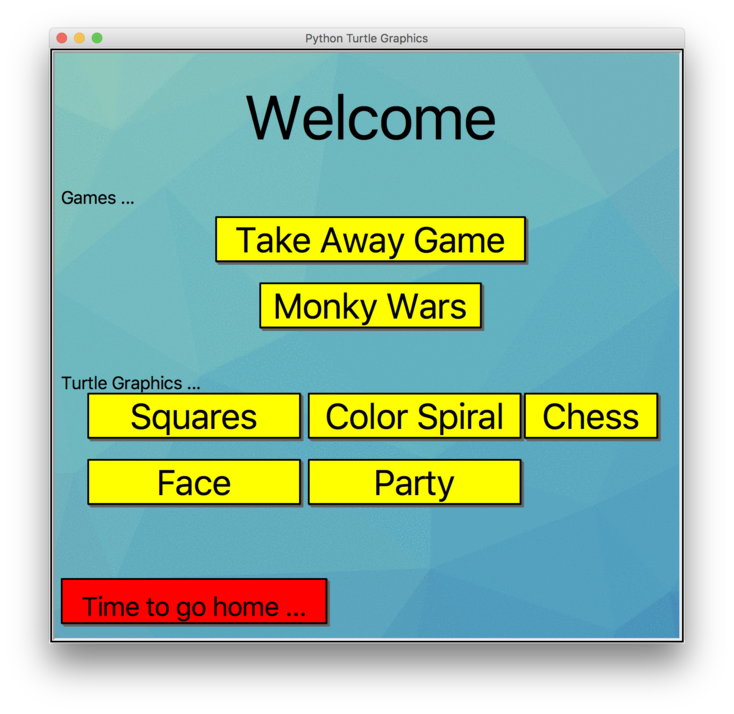
\includegraphics[width=6cm]{Menu_Complete}\\[-12pt]
\caption{Completed main menu.} 
\end{figure}
\end{minipage}

\vspace{6pt}
As usual we build this using a sequence of steps --- testing our code along the way.

\begin{dingautolist}{192} 
\contentsitem{screen}{Creating the Menu Screen}

We have done this many time before. All we need do is import the \code{turtle} module and create a \code{Screen} where we place our drawing, and a \code{Turtle} or two to do the actual drawing.  We do one thing that is new --- we insert a background image (must be in \code{gif} format).

\contentsitem{button}{Creating Buttons that Work}

Here we need to do some fancy coding --- both in drawing our buttons and figuring out how to respond to a button click.  

\contentsitem{take_away}{Building the Menu}

Finally, here you can design your menu screen anyway you want --- don't be stuck with my boring, everything is in a gird layout.

\contentsitem{button}{Updating our Earlier Programs so they Behave with Our Menu --- TODO}

We will need to modify some of our earlier programs (Graphical Take Away, Monkey Wars, etc) so they work better when we run them from our menu.  

This is a small task that we will leave until next week. Also we have yet to add the cool features!

\end{dingautolist}

\clearpage
\section{Creating the Menu Screen}\label{sec:screen}

\TODO{Create file called \code{Menu.py} and insert the following code.}

\codeonly{title={\code{Menu.py}}}{1}{120}{code}{Menu_Start.py}  
\mbox{}\hfill\raisebox{4cm}[0pt][0pt]{%
	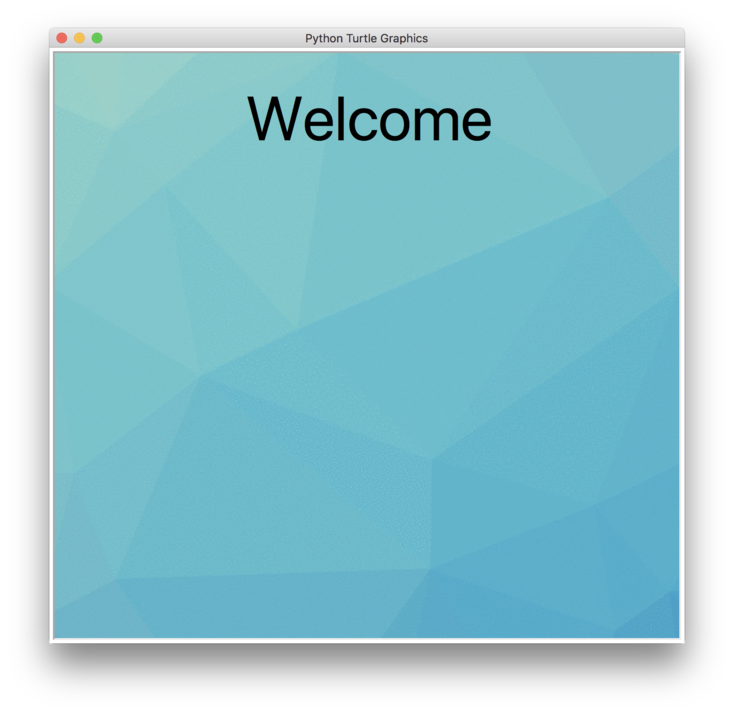
\includegraphics[width=9cm]{Menu_Start}
}\hspace*{-1.5cm}

Our code will get long so we need to keep things organised. Here the code is divided in to four sections --- import modules, create the empty screen and set background, define helper functions, and finally build the screen.

Currently this code just creates the window with the ``Welcome'' message. Next we will add buttons and mouse click events.
\clearpage

\section{Creating Buttons that Work}\label{sec:buttons}

\begin{figure}[H]
\centering\larger[2]\vspace{-18pt}
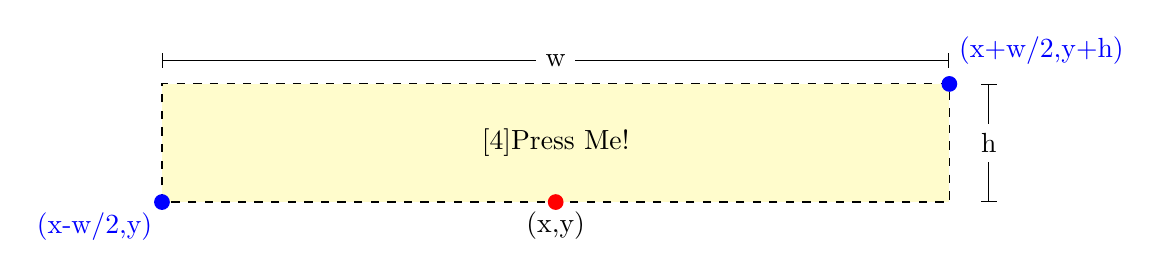
\begin{tikzpicture}
	\draw[dashed,fill=yellow!20] (-5,0) rectangle (5,1.5);
	\fill[red] (0,0) circle (.1) node[below,black] {(\code{x},\code{y})};
	
	\node[font={\larger[4]}]  at (0,0.75) {Press Me!};
	\draw[|-|] (5.5,0) -- node[fill=white] {\code{h}} ++(0,1.5); 
	\draw[|-|] (-5,1.8) -- node[fill=white] {\code{w}} ++(10,0); 
	\fill[blue] (-5,0) circle (.1) node[below,left,yshift=-9pt] {(\code{x}-\code{w/2},\code{y})};
	\fill[blue] (5,1.5) circle (.1) node[above,right,yshift=12pt] {(\code{x+w/2},\code{y+h})};
\end{tikzpicture}
\caption{Button position and dimensions.\label{fig:button}}
\end{figure}

\subsection{Developing a function to build a Button}

In order to create a button that we can click we need to decide on its:
\begin{itemize}
\item Position\footnote{Remember how we navigate across the screen
\begin{itemize}
\item
The centre, also called the {\bf origin}, and is denoted by $(0,0)$.
\item
Every point on the screen is defined by two numbers, $(x,y)$, where $x$ = how far to the right of the origin and $y$ = how far above the origin.
\end{itemize}} on the screen, (\code{x,y})

{\em We want the button text to be centred and draw the rectangle around the text so we will position a button based on the centre of the bottom edge (see Figure~\ref{fig:button})}.

\item Width, (\code{w}), and height, (\code{h}).

{\em
We need to draw a box big enough so that it looks like the text is inside this. If we used a GUI library this would be done automatically but we will do this manually and just pick numbers for now.}

\item Button label, (\code{label})

{\em This will be the text that the user sees and also the name of the button when we are responding to events.}

\item Font, (\code{font})

{\em
We might want the more important buttons to use a larger font so we need to be able to set this.}

\end{itemize}

Since we are planning to create multiple buttons we should write a function that we can call for every button.

\TODO{At the bottom of the ``\code{Define helper functions}''  section of your code insert the following function. }  

\codeonly{title={\code{Menu.py}}}{31}{38}{code}{Menu_1.py}  

In the above code, we have given default values for every parameter --- this will simplify our code later.

\TODO{After the ``Welcome'' message code in the ``\code{Build sceen}''  section, try to create a few buttons using the following code:} 
 
\codeonly{title={\code{Menu.py}}}{48}{50}{code}{Menu_1.py}  

\TODO{Run your code} 

You should see nothing on the screen, but see three messages in Thonny saying  

\begin{verbatim}
Button `Press Me` Not done yet
Button `No Press Me` Not done yet
Button `Forget them, PRESS ME` Not done yet
\end{verbatim}

Now we are going to implement our button function \ldots

\subsubsection{Draw the button label}

\vspace{6pt}

\TODO{After the  ``\code{draw label}'' comment insert code that jumps \code{bob} to correct position and writes the button label. Run this and you should see the labels.}

\codeonly{title={\code{Menu.py}}}{36}{38}{code}{Menu_2.py}  
\mbox{}\hfill\raisebox{0cm}[0pt][0pt]{%
	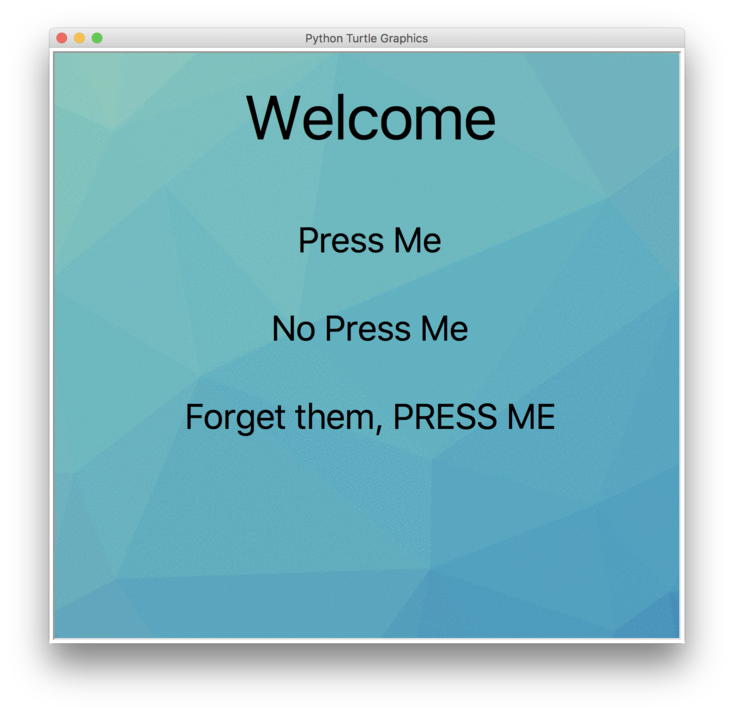
\includegraphics[width=4cm]{Menu_2}
}\hspace*{-1.5cm}

This looks good. Lets now add a border \ldots 

\subsubsection{Draw the border}

\TODO{After the  ``\code{draw border}'' comment insert code that draws a 
rectangle of width \code{w}, and height \code{h}}

\codeonly{title={\code{Menu.py}}}{40}{45}{code}{Menu_3.py}  
\mbox{}\hfill\raisebox{0.5cm}[0pt][0pt]{%
	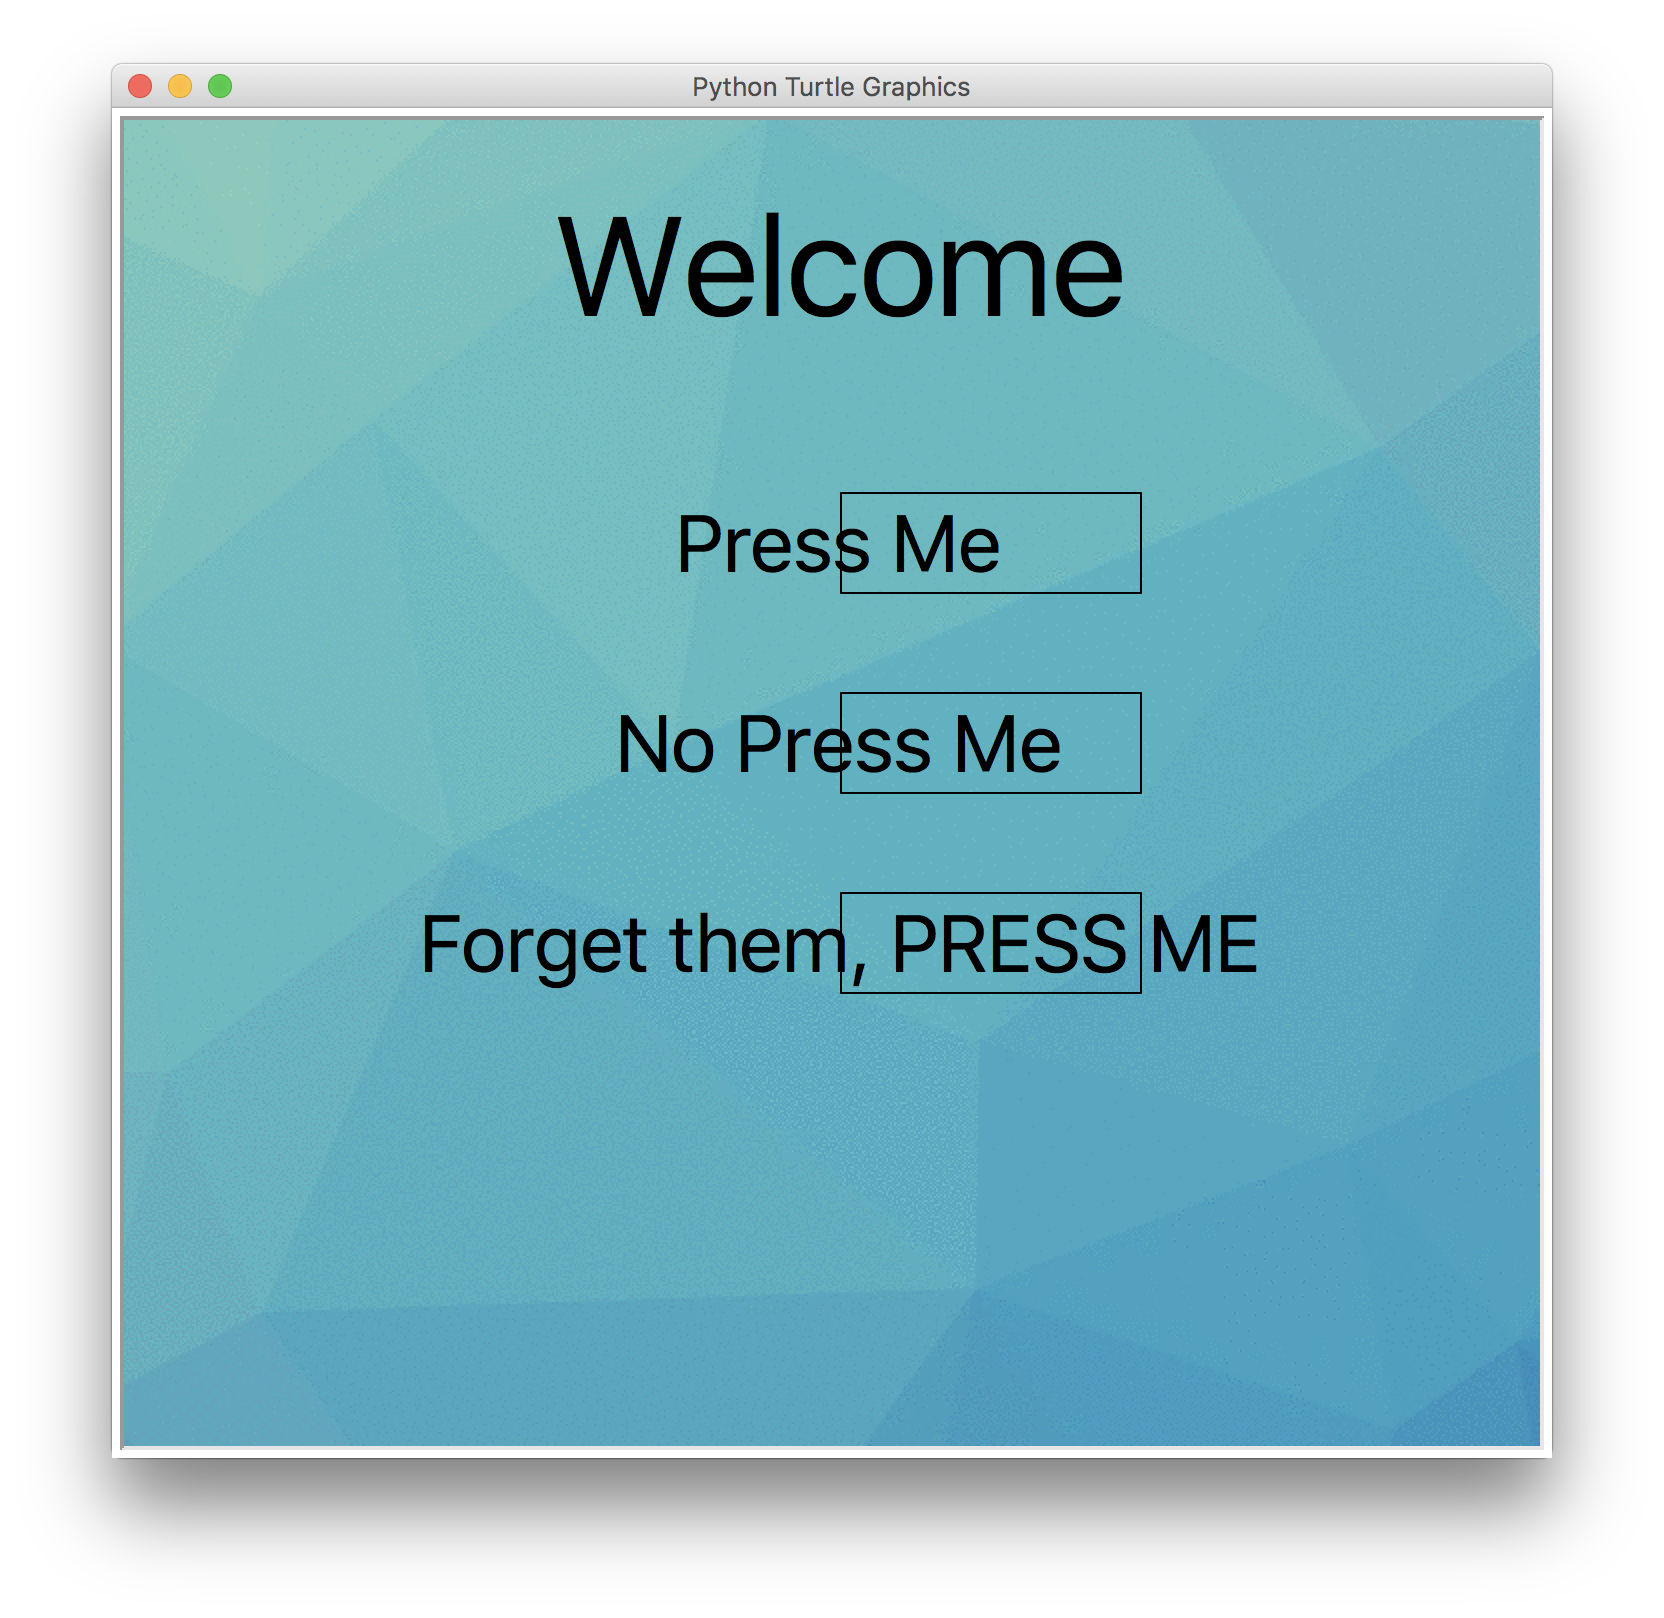
\includegraphics[width=4cm]{Menu_3}
}\hspace*{-1.5cm}

I see two problems here. The width of the rectangles is too small --- this is easy to fix. We just set the \code{w} parameter when calling \code{drawButton}. The second problem is that the rectangle is drawn starting from the bottom centre of the label --- we fix this by moving \code{bob} to the bottom left corner (see Figure~\ref{fig:button}).

\TODO{Insert code to move \code{bob} to bottom left corner, and change the widths of the 
button in your \code{drawButton} calls by setting parameter \code{w}. You should then get the following.}

\codeonly{title={\code{Menu.py}}}{40}{46}{code}{Menu_4.py}  
\mbox{}\hfill\raisebox{0.5cm}[0pt][0pt]{%
	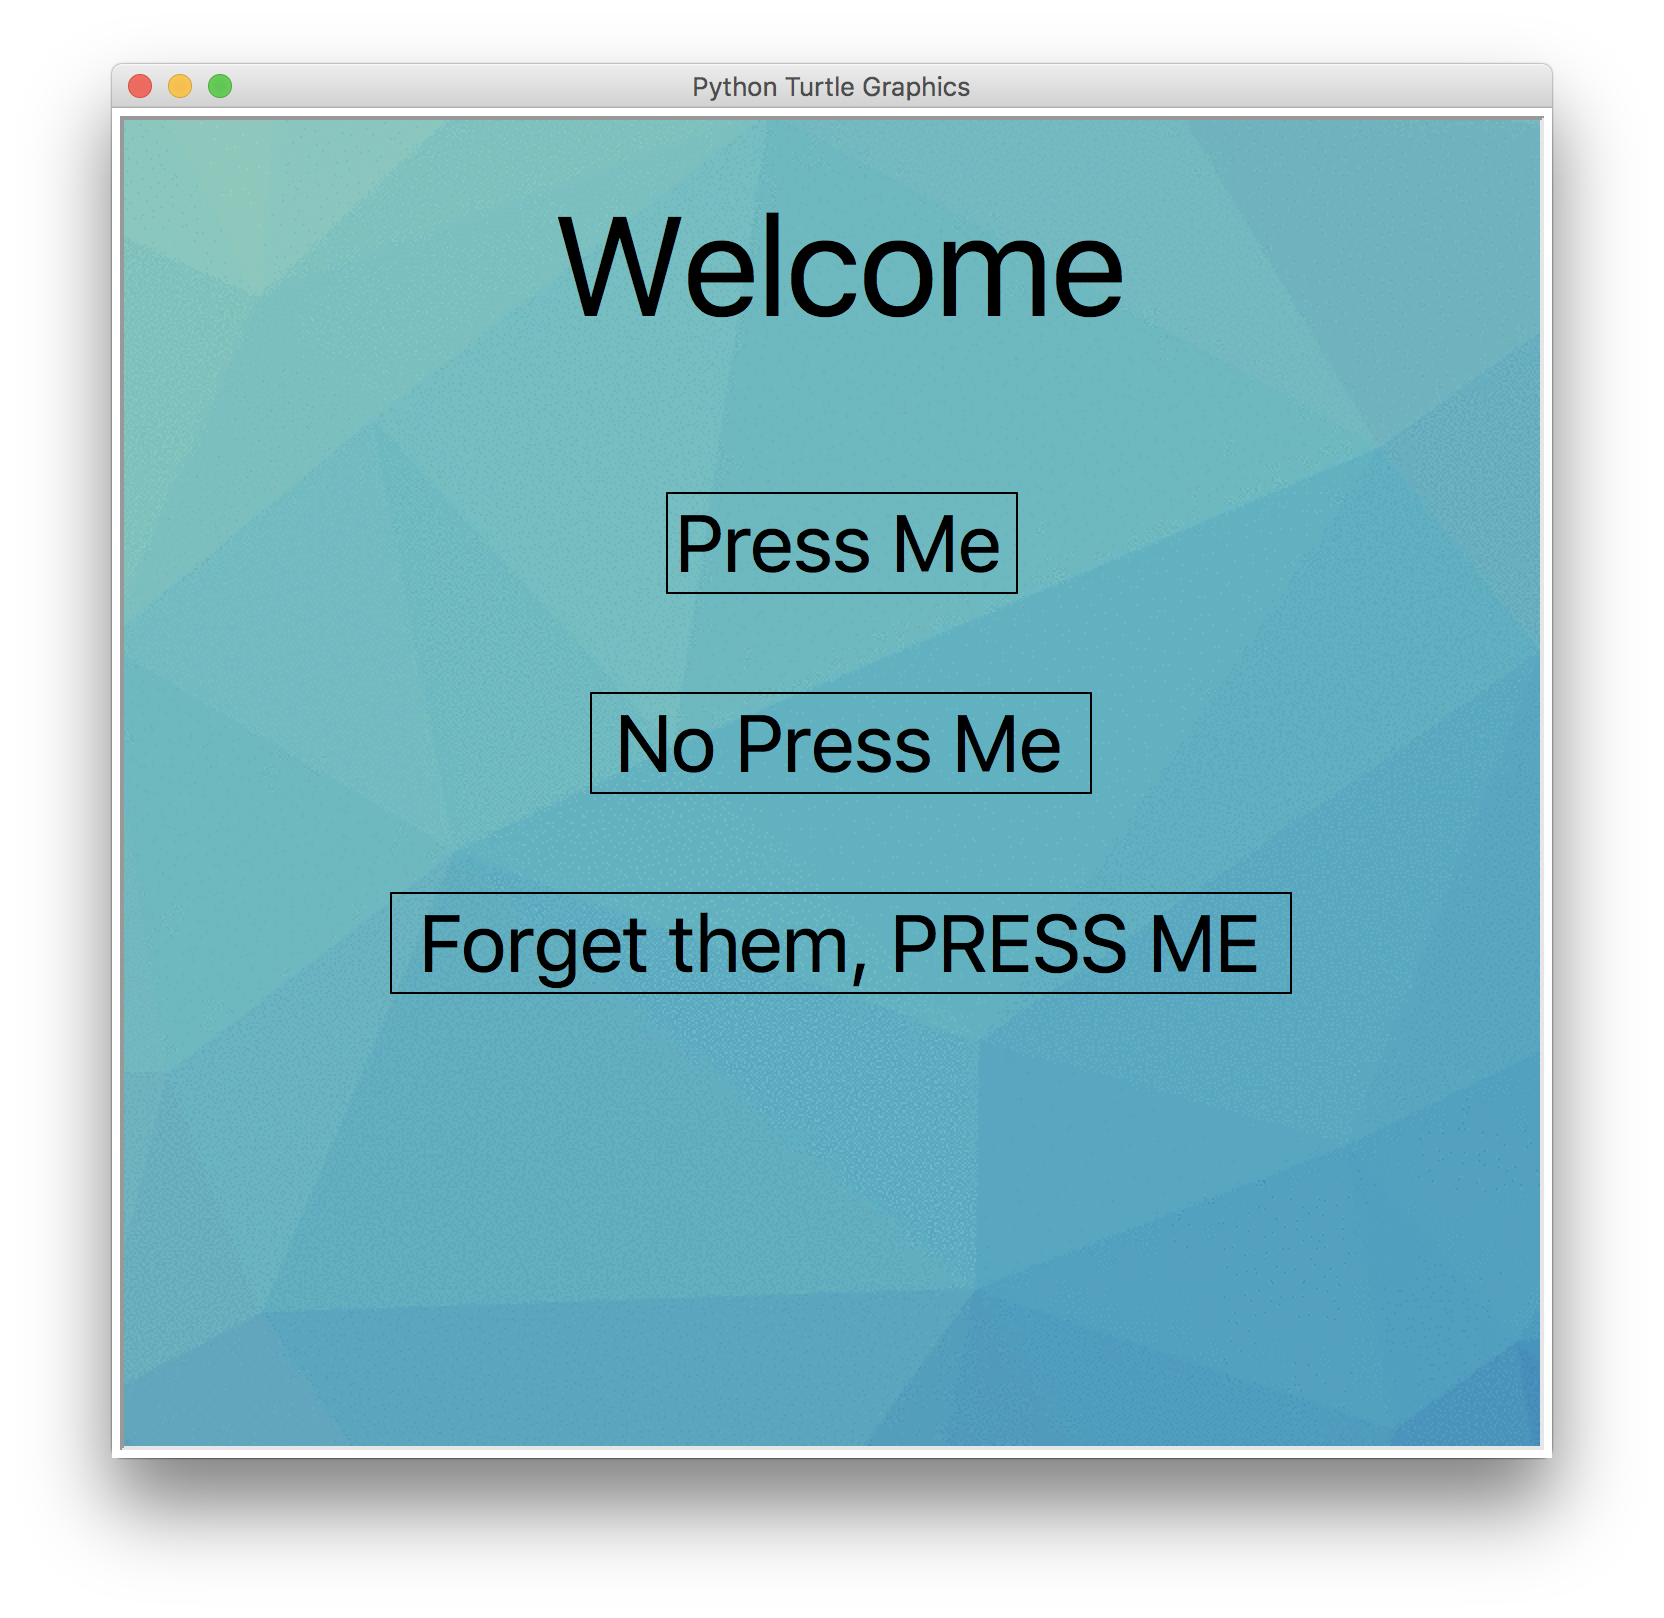
\includegraphics[width=4cm]{Menu_4}
}\hspace*{-1.5cm}

Now the above works, but putting basic drawing of a rectangle inside our draw button is not a great idea.  We will be drawing lots of rectangles so lets move that code out into a new helper function.

\TODO{Before your \code{drawButton} function in \code{Define helper functions} section, insert the following function}

\codeonly{title={\code{Menu.py}}}{31}{46}{code}{Menu_5.py}  

This function will draw a rectangle of width \code{w}, and height \code{h}, with bottom left corner at position (\code{x},\code{y}). You can also specify the border colour and the fill colour.

\vspace{12pt}

You should think about extending this function by, for example,
\begin{itemize}
\item Adding parameter \code{pensize=2} which would set the thickness of the border.
\item Adding parameter \code{shadow=False} which when set to \code{True} would draw a shadow. 

Drawing a shadow, is actual easy --- we just draw a few rectangles a little to the right an a little below the position of the main rectangle BEFORE we draw the main rectangle. If you are exceedingly lazy (this is a good thing in a programmer!) you can draw the shadow rectangles by just calling the \code{drawRectangle} function from inside the  \code{drawRectangle}
\end{itemize}
\newpage

Now your \code{drawButton can be simplified to}

\codeonly{title={\code{Menu.py}}}{49}{59}{code}{Menu_5.py}
\mbox{}\hfill\raisebox{0.85cm}[0pt][0pt]{%
	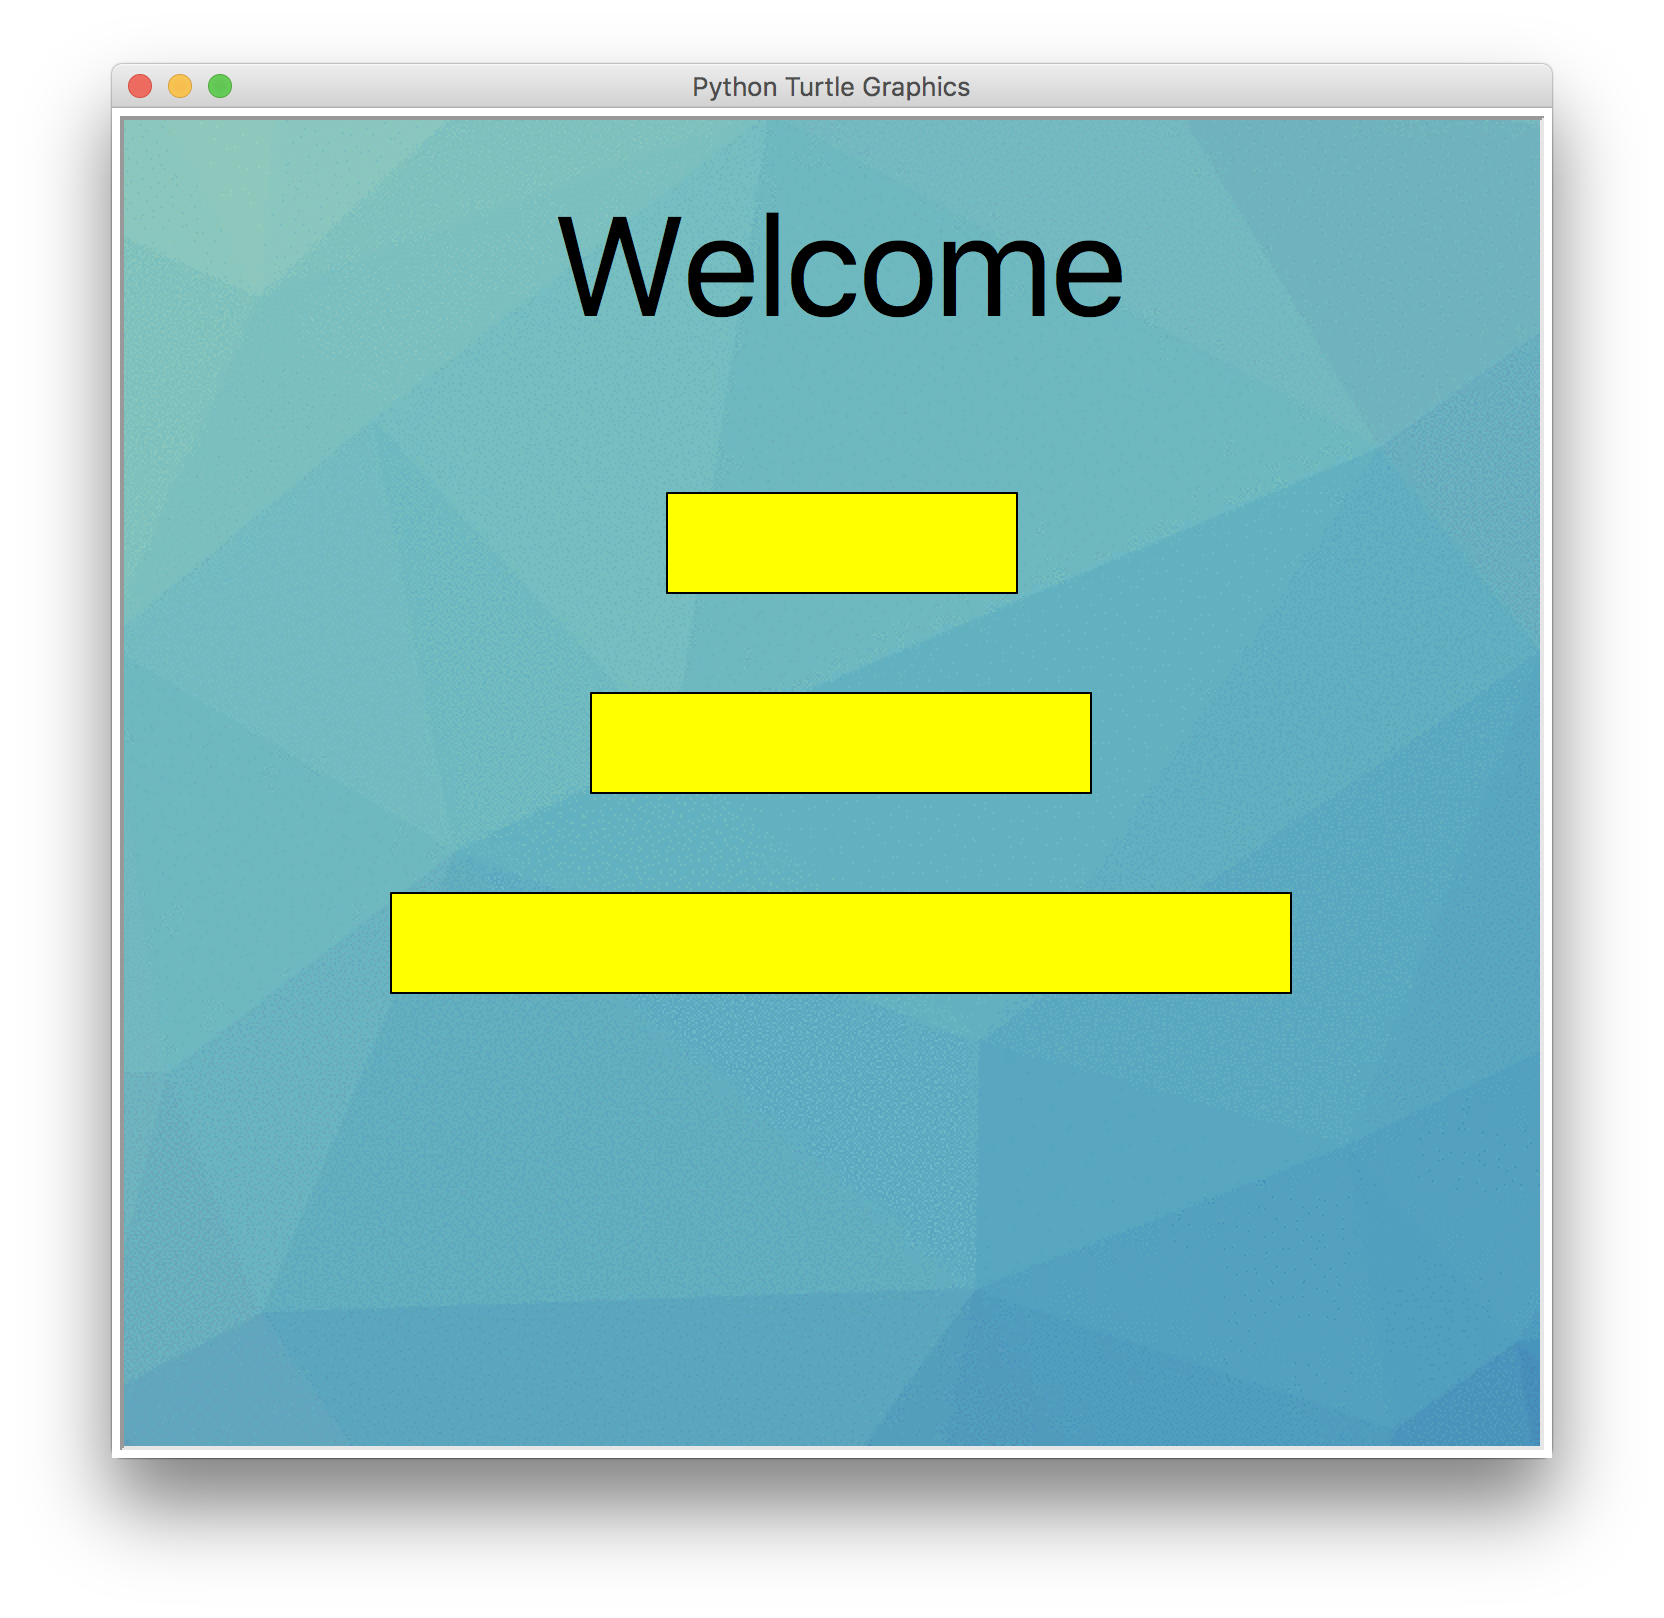
\includegraphics[width=4cm]{Menu_5}
}\hspace*{-1.5cm}

\TODO{If you look, really really carefully at the output you will see that {\em we} have done something silly.  To fix this, we need to draw the button label after drawing the border. Fix This.}

\codeonly{title={\code{Menu.py}}}{54}{64}{code}{Menu_6.py}
\mbox{}\hfill\raisebox{0.85cm}[0pt][0pt]{%
	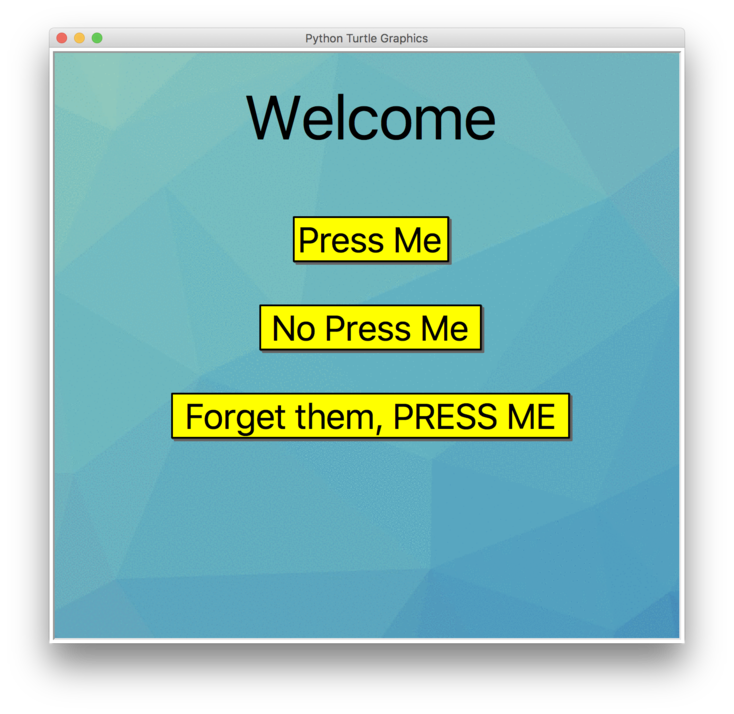
\includegraphics[width=4cm]{Menu_6}
}\hspace*{-1.5cm}


\subsubsection{Making the buttons work}

OK, now we have things that looks like buttons, but they do not act like them --- click on a button and see what happens --- nothing. 

To get the buttons to work we need to do two things:

\begin{itemize}
\item Listen for and respond to click events.

This is easy --- we will create our own \code{onclick} function to run whenever the user clicks on the screen.

\item When a click occurs, decide whether it happened within a button region and which button.

This is a little harder so we will talk about this in some detail.
\end{itemize}

\newpage

\TODO{Insert the following function at the bottom of the ``\code{Define helper functions}'' section of your code.}

\codeonly{title={\code{Menu.py}}}{67}{69}{code}{Menu_7.py}

and just before the \code{turtle.mainloop()} insert the lines

\codeonly{title={\code{Menu.py}}}{84}{85}{code}{Menu_7.py}

Now run your code and make sure you see a message appearing in {\em Thonny} every time you click the left mouse button. You should see that you also get the position of the mouse in the screen when the click occurred. Next we need to use this position information to determine which button was ``pressed''.

\TODO{Insert the code at the bottom of the ``\code{Create screen}'' section of your code.}

\codeonly{title={\code{Menu.py}}}{21}{23}{code}{Menu_8.py}

\begin{itemize}
\item
Lines 21 and 22, allow us to create an object (like the \code{Turtle} object or the \code{Screen} object) which stores information for a Button. Our \code{Button} object stores position (\code{x},\code{y}), size  \code{w} by \code{h}, and \code{label}.
\item
Line 23 defines an empty list, called \code{buttons}, that will store the information for all generated buttons.
\end{itemize}

So where do we get the information that we want to store in the \code{buttons} list?  

We have this information at end of \code{drawButton} function so that is where we will build our \code{Button} object.

\TODO{Modify the \code{drawButton} function so that it returns a \code{Button} object, as shown below.}
 
\codeonly{title={\code{Menu.py}}}{58}{69}{code}{Menu_8.py}

Now \code{bob} has a list of all of the generated buttons which we can search whenever the user clicks on the screen. First we need to make sure we are happy with our geometry. The mouse click is recorded at the point (\code{mx},\code{my}).  The conditions that must be true if this point is inside a button rectangle are shown in the following figure.

\begin{figure}[H]
\centering\larger[2]\vspace{-18pt}
\begin{tikzpicture}
	\draw[dashed,fill=yellow!20] (-5,0) rectangle (5,1.5);
	\fill[red] (0,0) circle (.1) node[below,black] {(\code{x},\code{y})};
	
	%\node[font={\larger[4]}]  at (0,0.75) {Press Me!};
	\draw[|-|] (5.5,0) -- node[fill=white] {\code{h}} ++(0,1.5); 
	\draw[|-|] (-5,1.8) -- node[fill=white] {\code{w}} ++(10,0); 
	\fill[blue] (-5,0) circle (.1) node[below,left,yshift=-9pt] 
	{(\code{x}-\code{w/2},\code{y})};
	\fill[blue] (5,1.5) circle (.1) node[above,right,yshift=12pt] {(\code{x+w/2},\code{y+h})};
	
	\fill[green!80!black] (3,1) circle (.1) node[below left,black] {(\code{mx},\code{my})};
	
	\draw[decorate,decoration={brace,amplitude=10pt}] (5,-1) -- 
	node[below, yshift=-15pt,fill=white,draw,drop shadow] 
	{\code{x}-\code{w/2 < mx <  x+w/2}}
	++(-10,0);

	\draw[decorate,decoration={brace,amplitude=10pt}] (-5.5,0) -- 
	node[left, xshift=-15pt, fill=white,draw,drop shadow] 
	{\code{y < my <  y+h}}
	++(0,1.5);
	
\end{tikzpicture}
\caption[Given button and point, determine if point is inside button]{Given a button and a point (\code{mx},\code{my}), determine if point is inside button.\label{fig:button}}
\end{figure}

\TODO{Modify your \code{onclick} function so that it check every button stored in \code{bob.buttons} using the conditions on (\code{mx},\code{my}) shown in the above figure.\\

Run this code and verify that whenever you click on a button that button's label is printed.
}

\codeonly{title={\code{Menu.py}}}{72}{78}{code}{Menu_8.py}


So finally we want to run different code depending on which button has been pressed. To do this we check the label of the button.

\TODO{Update the \code{onclick} function as shown below.}

\codeonly{title={\code{Menu.py}}}{72}{87}{code}{Menu_9.py}

\subsection{It's Lego time --- Putting your Programs Together}

OK, we now have nearly everything to build our menu. To get the menu layout that I showed at the start of this worksheet I used the following code.  You don't have to follow this.

\codeonly{title={\code{Menu.py}}}{99}{118}{code}{Menu_10.py}
\mbox{}\hfill\raisebox{7cm}[0pt][0pt]{%
	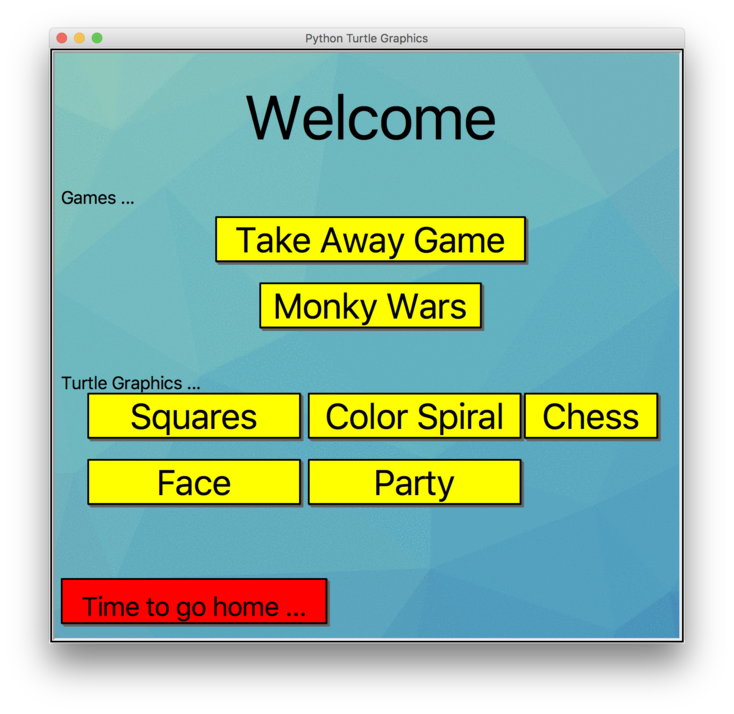
\includegraphics[width=6cm]{Menu_Complete}
}\hspace*{-1.5cm}

Then in my \code{onclick} functions I have added {\bf some} of the code needed to respond to the above button clicks.
 
\codeonly{title={\code{Menu.py}}}{72}{89}{code}{Menu_10.py}

Notice in line 80 and in line 83 I run other python files.  You will need to change this to match the name that you used for your files.
\end{document}




